\begin{figure}[H]
    \centering
    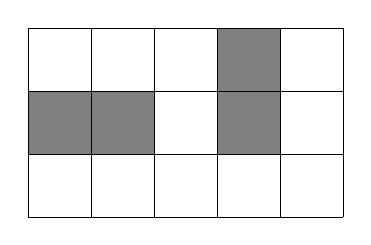
\begin{tikzpicture}[scale=0.8]
        \foreach \x in {0,...,4} {
            \foreach \y in {0,...,2} {
                \fill[gray] (\x,\y) rectangle ++(1,1);
            }
        }
        \fill[white] (0, 2) rectangle ++(1,1);
        \fill[white] (1, 2) rectangle ++(1,1);
        \fill[white] (2, 2) rectangle ++(1,1);

        \fill[white] (0,0) rectangle ++(1,1);
        \fill[white] (2,0) rectangle ++(1,1);
        \fill[white] (2,1) rectangle ++(1,1);
        \fill[white] (3,0) rectangle ++(1,1);
        \fill[white] (4,0) rectangle ++(1,1);
        \fill[white] (4,1) rectangle ++(1,1);
        \fill[white] (4,2) rectangle ++(1,1);
        \fill[white] (1,0) rectangle ++(1,1);

        \draw[step=1cm,ultra thin,black] (0,0) grid (5,3);
    \end{tikzpicture}
    \caption{\centering Końcowy wygląd labiryntu. Pozostałe powroty nie wygenerowały żadnych przejść ze względu na brak prawidłowych ruchów.}
    \label{fig:dfs_gen_step_8}
\end{figure}